%
% @author   Shmish  "shmish90@gmail.com"
% @legal    MIT     "(c) Christopher Schmitt"
%


\documentclass{article}


%
% Document Imports
%

\usepackage{fancyhdr}
\usepackage{extramarks}
\usepackage{amsmath}
\usepackage{amssymb}
\usepackage{amsthm}
\usepackage{amsfonts}
\usepackage{color}
\usepackage{tikz}
\usepackage{algorithmicx}
\usepackage[noend]{algpseudocode}
\usepackage{algorithm}
\usepackage{tikz-qtree}



%
% Document Configuration
%

\newcommand{\hwAuthor}{Christopher K. Schmitt}
\newcommand{\hwSubject}{CS 407}
\newcommand{\hwSection}{Section 02}
\newcommand{\hwSemester}{Spring 2021}
\newcommand{\hwAssignment}{Midterm}


%
% Document Environments
%

\setlength{\headheight}{65pt}
\pagestyle{fancy}
\lhead{\hwAuthor}
\rhead{
  \hwSubject \\
  \hwSection \\
  \hwSemester \\
  \hwAssignment
}

\newenvironment{problem}[1]{
  \nobreak\section*{Problem #1}
}{}

\newcommand*{\Let}[2]{\State #1 $\gets$ #2}
\newcommand*{\bigO}[1]{\ensuremath{\mathcal{O}\left(#1\right)}}
\newcommand*{\bigTheta}[1]{\ensuremath{\Theta\left(#1\right)}}
\newcommand*{\bigOmega}[1]{\ensuremath{\Omega\left(#1\right)}}


%
% Document Start
%

\begin{document}
  \begin{problem}{1.1}
    \begin{verbatim}
@base <https://shmishtopher.github.io#>.
@prefix rdf: <http://www.w3.org/1999/02/22-rdf-syntax-ns#>.

:bob :believes [
  rdf:type      rdf:Statement;
  rdf:subject   :carly;
  rdf:predicate :loves;
  rdf:object    :bob
].
    \end{verbatim}
  \end{problem}

  \begin{problem}{1.2}
    \begin{verbatim}
@base <https://shmishtopher.github.io#>.
@prefix rdf: <http://www.w3.org/1999/02/22-rdf-syntax-ns#>.

:teacher :notices [
  rdf:type      rdf:Statement;
  rdf:subject   :john;
  rdf:predicate :worksOn;
  rdf:object    :project
].
    \end{verbatim}
  \end{problem}

  \pagebreak
  \begin{problem}{2.1}
    \begin{verbatim}
PREFIX ex: <http://example.org/>

SELECT ?body WHERE {
  { 
    ex:Sun ex:satellite ?body.
  } 
  
  UNION
  
  {
    ex:Sun ex:satellite ?child.
    ?child ex:satellite ?body.
  }
}
    \end{verbatim}

    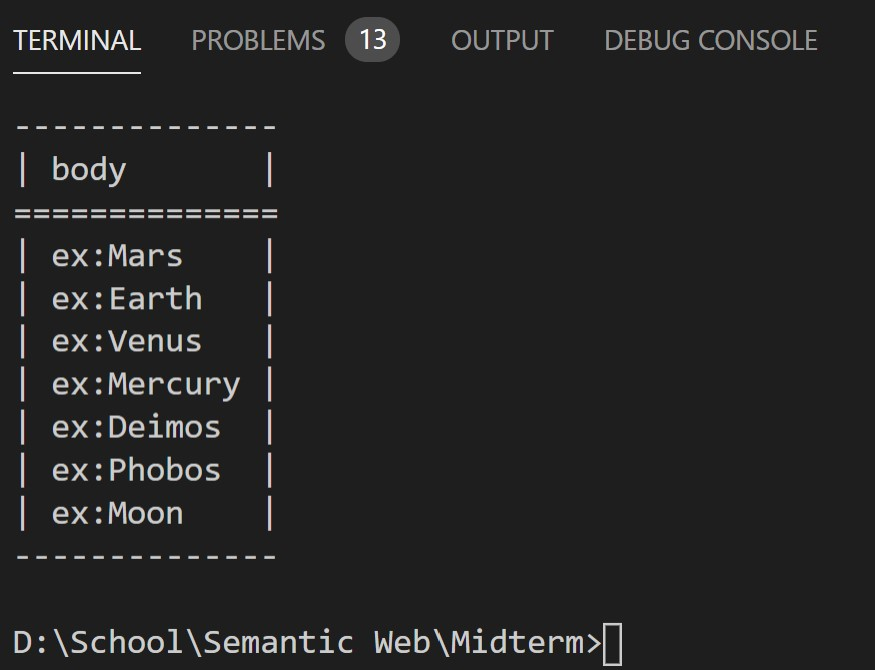
\includegraphics{images/0.jpg}
  \end{problem}

  \pagebreak
  \begin{problem}{2.2}
    \begin{verbatim}
PREFIX ex: <http://example.org/>

SELECT ?body ?parent {
  ?body ex:radius ?radius.
  
  FILTER(?radius > 1683.89).
  
  OPTIONAL { 
    ?parent ex:satellite ?body.
  }
}
    \end{verbatim}
    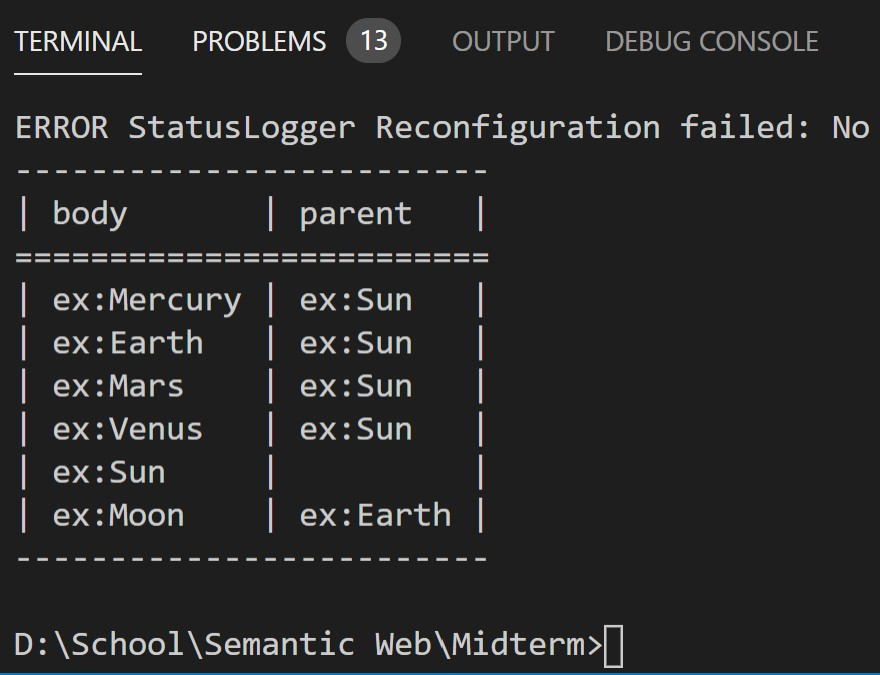
\includegraphics{images/1.jpg}
  \end{problem}

  \pagebreak
  \begin{problem}{2.3}
    \begin{verbatim}
PREFIX ex: <http://example.org/>

SELECT DISTINCT ?body {
  ?body ex:satellite ?satellite.
  ?parent ex:satellite ?body.
  ?parent ex:radius ?radius.
  ?satellite ex:name ?name.
  
  FILTER(?radius > 1500 && lang(?name) = 'en').
}
    \end{verbatim}

    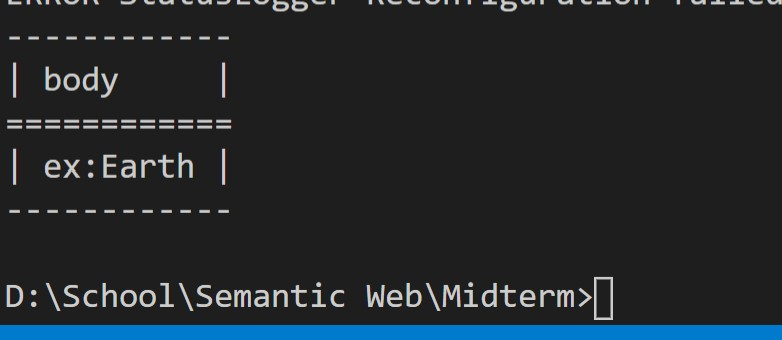
\includegraphics{images/2.jpg}
  \end{problem}

  \begin{problem}{2.4}
    \begin{verbatim}
PREFIX ex: <http://example.org/>

SELECT ?body (COUNT(?satellite) as ?count) WHERE {
  ?body ex:satellite ?satellite.
}
GROUP BY ?body
HAVING (?count > 1)
    \end{verbatim}

    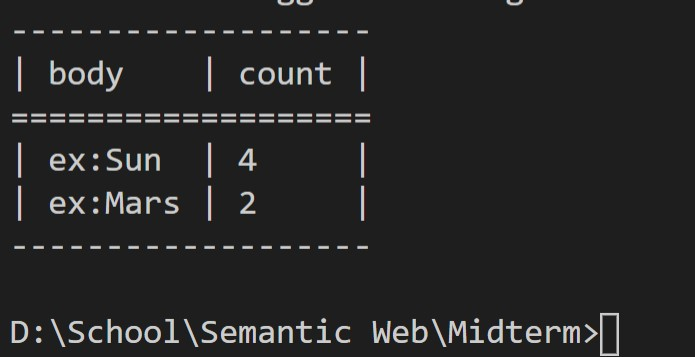
\includegraphics{images/3.jpg}
  \end{problem}

  \begin{problem}{3}
    The following file is also included as an
    \begin{verbatim}
@base <https://shmishtopher.github.io#>.
@prefix rdfs: <http://www.w3.org/2000/01/rdf-schema#>.

#
# Films
#
:Giant
  :year 1956;
  :directedBy :FredGuiol;
  :starring
    :ElizabethTaylor,
    :RockHudson,
    :JamesDean.

:EastOfEden
  :year 1955;
  :directedBy :EliaKazan;
  :starring
    :JamesDean,
    :RaymondMassey,
    :JulieHarris.

:ItShouldHappenToYou
  :year 1954;
  :directedBy :GeorgeCukor;
  :starring
    :JudyHolliday,
    :JackLemmon,
    :PeterLawford.

:TheSearchers
  :year 1956;
  :directedBy :JohnFord;
  :starring
    :JohnWayne,
    :JefferyHunter,
    :VeraMiles.

:RebelWithoutACause
  :year 1955;
  :directedBy :NicholasRay;
  :starring
    :JamesDean,
    :NatalieWood,
    :SalMineo.

#
# Directors
#
:FredGuiol
  a :Director;
  rdfs:label "Fred Guiol".

:EliaKazan
  a :Director;
  rdfs:label "Elia Kazan".

:GeorgeCukor
  a :Director;
  rdfs:label "George Cukor".

:JohnFord
  a :Director;
  rdfs:label "John Ford".

:NicholasRay
  a :Director;
  rdfs:label "Nicholas Ray".

#
# Actors
#
:ElizabethTaylor
  a :Actor;
  rdfs:label "Elizabeth Talor".

:RockHudson
  a :Actor;
  rdfs:label "Rock Hudson".

:JamesDean
  a :Actor;
  rdfs:label "James Dean".

:RaymondMassey
  a :Actor;
  rdfs:label "Raymond Massey".

:JulieHarris
  a :Actor;
  rdfs:label "Julie Harris".

:JudyHolliday
  a :Actor;
  rdfs:label "Judy Holliday".

:JackLemmon
  a :Actor;
  rdfs:label "Jack Lemmon".

:PeterLawford
  a :Actor;
  rdfs:label "Perter Lawford".

:JohnWayne
  a :Actor;
  rdfs:label "John Wayne".

:JefferyHunter
  a :Actor;
  rdfs:label "Jeffery Hunter".

:VeraMiles
  a :Actor;
  rdfs:label "Vera Miles".

:NatalieWood
  a :Actor;
  rdfs:label "Natalie Wood".

:SalMineo
  a :Actor;
  rdfs:label "Sal Mineo".
    \end{verbatim}

    \pagebreak
    SELECT query 1:
    \begin{verbatim}
PREFIX : <https://shmishtopher.github.io#>

# Select all of the films starring James Dean
SELECT  ?film WHERE {
  ?film :starring :JamesDean.
}
    \end{verbatim}
    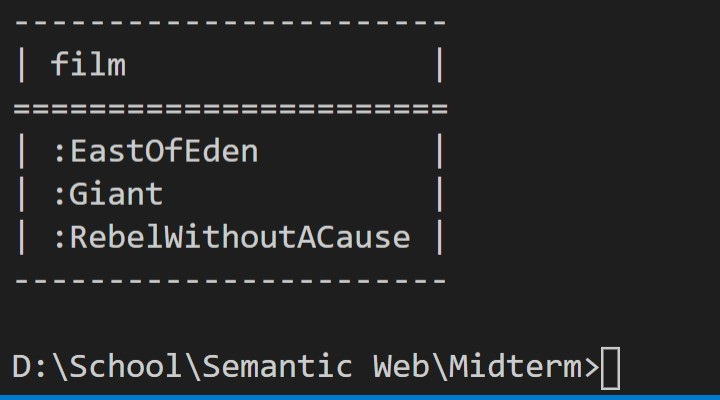
\includegraphics{images/4.jpg}

    SELECT query 2:
    \begin{verbatim}
PREFIX : <https://shmishtopher.github.io#>

# Select all of the films produced before 1956
SELECT  ?film ?year WHERE {
  ?film :year ?year.
  FILTER(?year < 1956).
}
    \end{verbatim}
    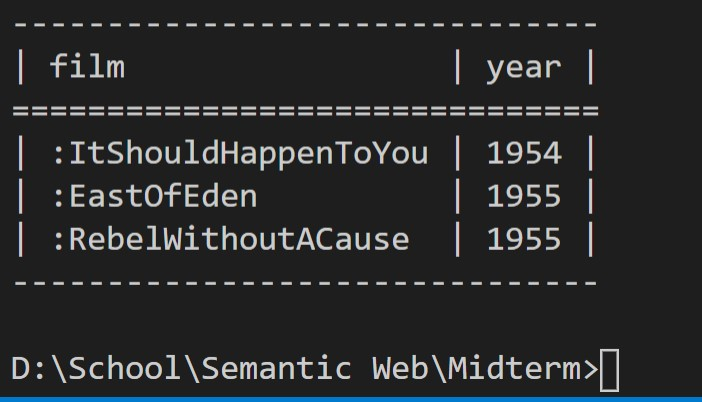
\includegraphics{images/5.jpg}

    \pagebreak
    SELECT query 3:
    \begin{verbatim}
PREFIX : <https://shmishtopher.github.io#>

# Select all of actors who have worked with James Dean
SELECT ?actor ?film WHERE {
  ?film :starring :JamesDean.
  ?film :starring ?actor.

  FILTER(?actor != :JamesDean).
}
    \end{verbatim}
    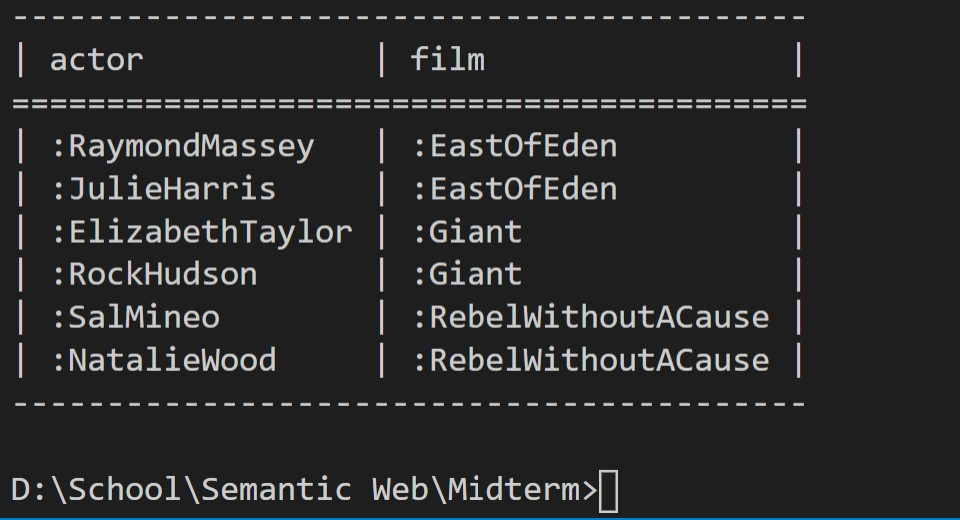
\includegraphics{images/6.jpg}

    \pagebreak
    CONSTRUCT query 1:
    \begin{verbatim}
PREFIX : <https://shmishtopher.github.io#>
PREFIX foaf: <http://xmlns.com/foaf/0.1/>

# Construct a graph of directors who know actors
CONSTRUCT { ?director foaf:knows ?actor } WHERE {
  ?film :directedBy ?director.
  ?film :starring ?actor.
}
    \end{verbatim}
    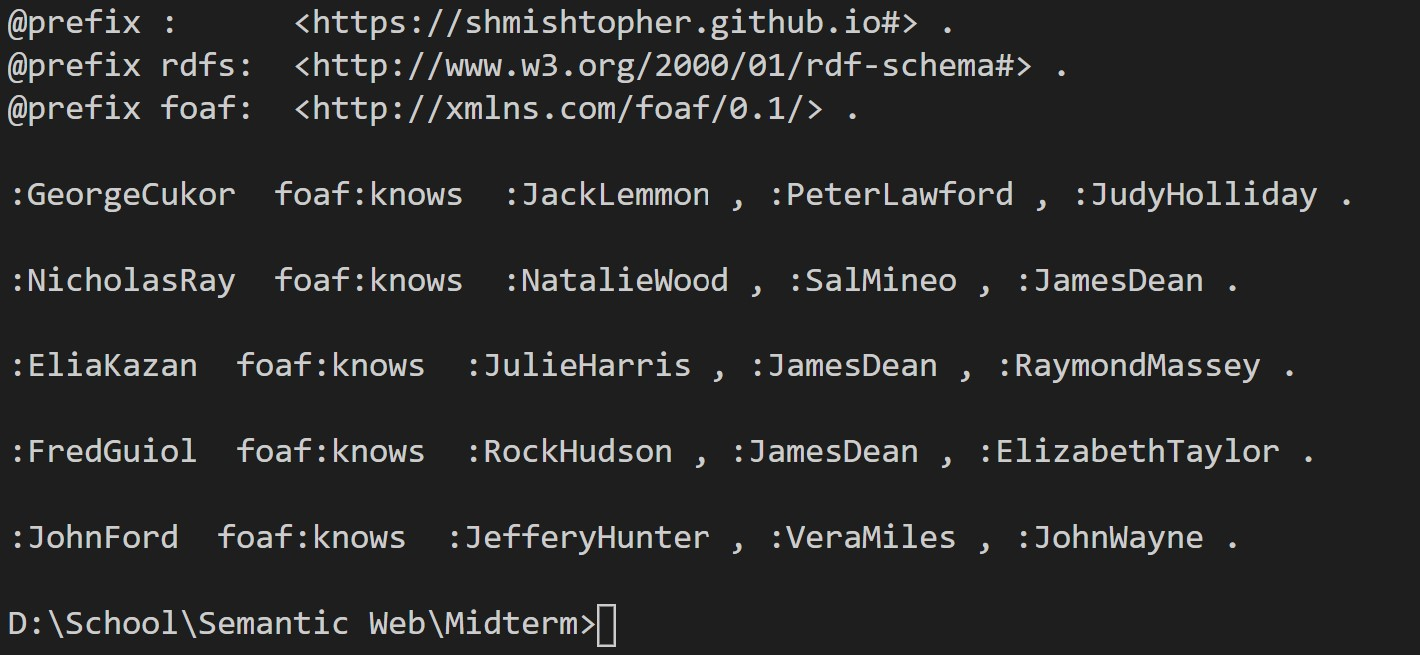
\includegraphics{images/7.jpg}

    \pagebreak
    CONSTRUCT query 2:
    \begin{verbatim}
PREFIX : <https://shmishtopher.github.io#>
PREFIX foaf: <http://xmlns.com/foaf/0.1/>

# Construct a graph of every actor who knows Fred Guiol
CONSTRUCT { ?actor foaf:knows :FredGuiol } WHERE {
  ?film :directedBy :FredGuiol.
  ?film :starring ?actor.
}
    \end{verbatim}
    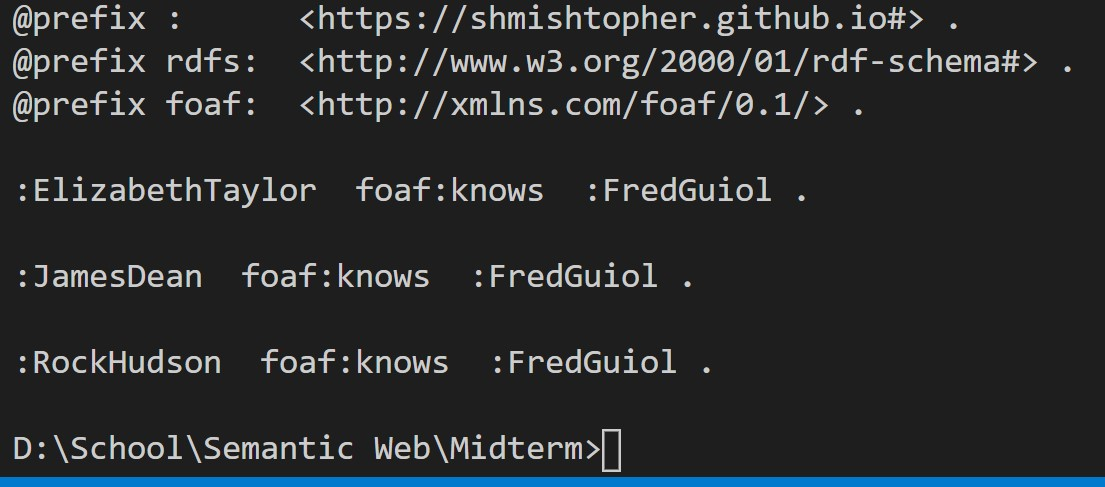
\includegraphics{images/8.jpg}

    ASK query:
    \begin{verbatim}
PREFIX : <https://shmishtopher.github.io#>

# Did Fred Guiol direct "Giant"?
ASK {
  :Giant :directedBy :FredGuiol.
}
    \end{verbatim}
    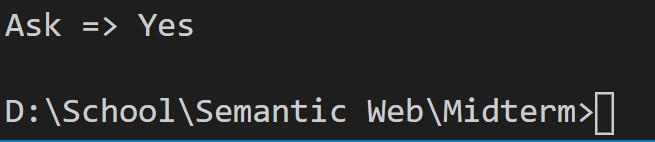
\includegraphics{images/9.jpg}
  

    \pagebreak
    DESCRIBE query:
    \begin{verbatim}
PREFIX : <https://shmishtopher.github.io#>

# Describe all the movies James Dean starred in
DESCRIBE ?x WHERE {
  ?x :starring :JamesDean.
}
    \end{verbatim}
    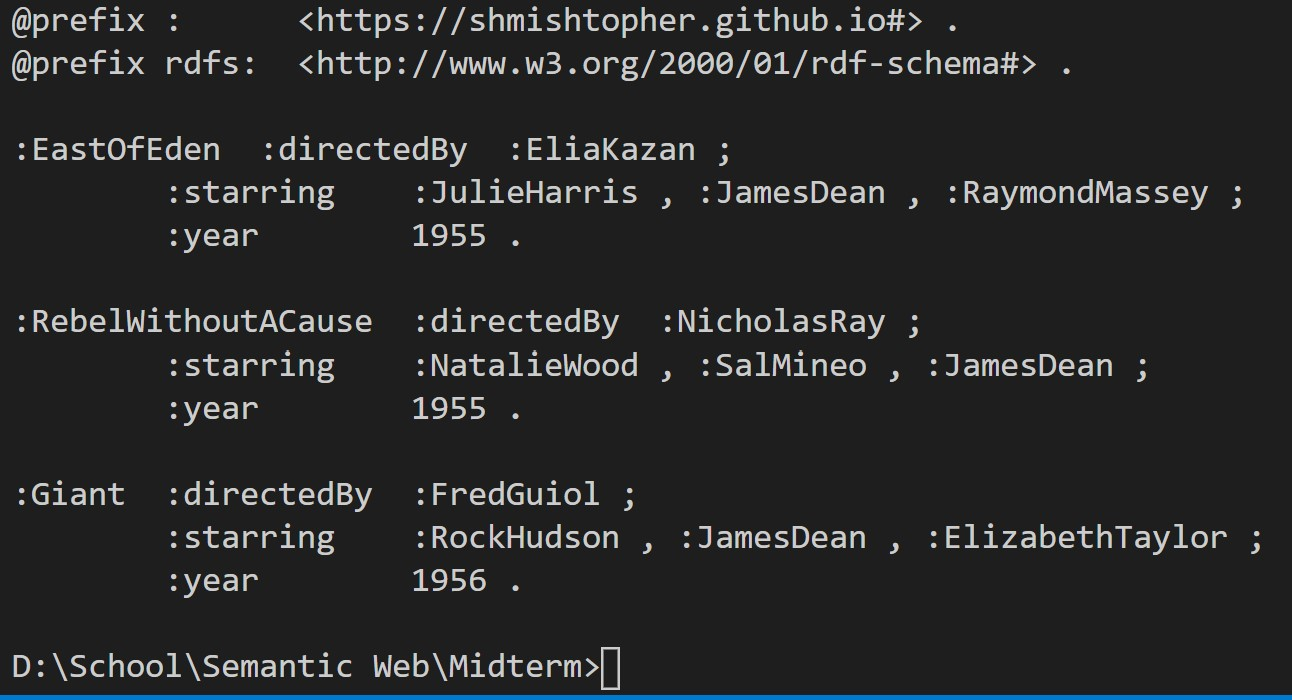
\includegraphics{images/10.jpg}
  \end{problem}

  \pagebreak
  \begin{problem}{4.1}
    \begin{verbatim}
PREFIX ex: <http://example.org/addressbook#>
PREFIX d: <http://example.org/data#>

INSERT DATA {
  d:i44
      ex:firstName "George";
      ex:lastName "Westerlund";
      ex:homeTel "(414) 344-1585";
      ex:email "GeorgeMWesterlund@gmail.com".
  
  d:i55
      ex:firstName "Elizabeth";
      ex:lastName "Holland";
      ex:homeTel "(802) 245-5788";
      ex:email "ElizabethMHolland@gmail.com".
}
    \end{verbatim}
  \end{problem}

  \pagebreak
  \begin{problem}{4.2}
    \begin{verbatim}
PREFIX ex: <http://example.org/addressbook#>
PREFIX d: <http://example.org/data#>

CONSTRUCT { 
  ?s a ex:Student.
  ?s ?p ?o.
}
WHERE { ?s ?p ?o }
    \end{verbatim}
    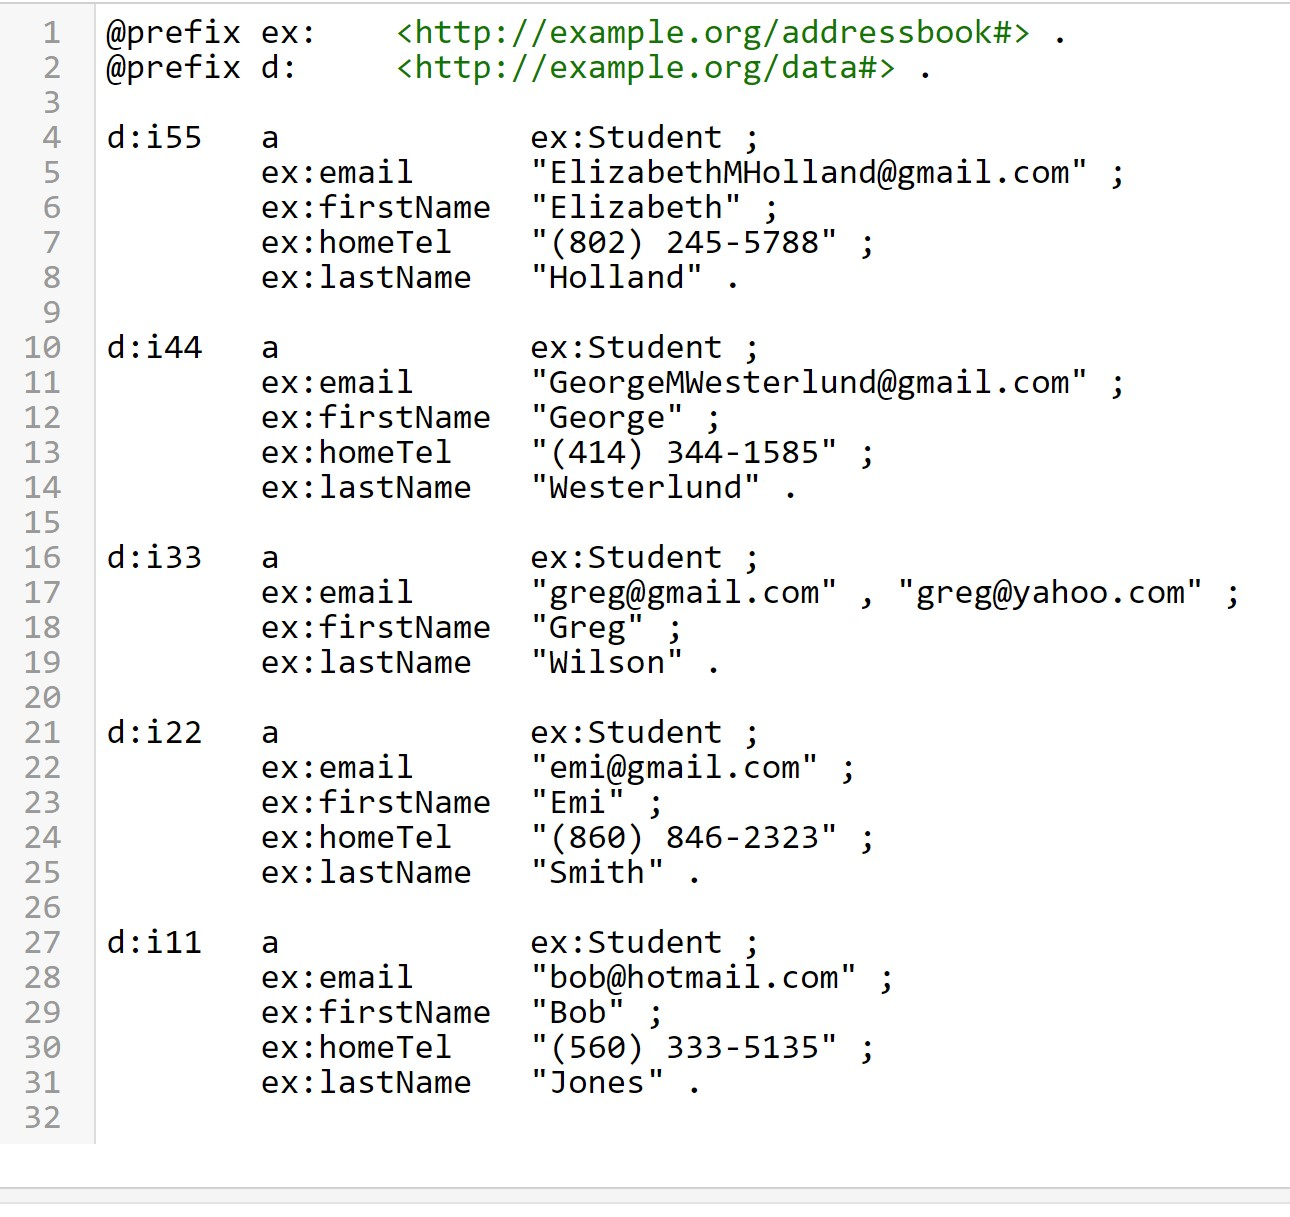
\includegraphics{images/11.jpg}
  \end{problem}

  \begin{problem}{4.3}
    \begin{verbatim}
PREFIX ex: <http://example.org/addressbook#>
PREFIX d: <http://example.org/data#>

SELECT DISTINCT ?first ?last { 
  ?x ex:firstName ?first.
  ?x ex:lastName ?last.
  
  FILTER NOT EXISTS { ?x ex:homeTel ?o }.
}
    \end{verbatim}

    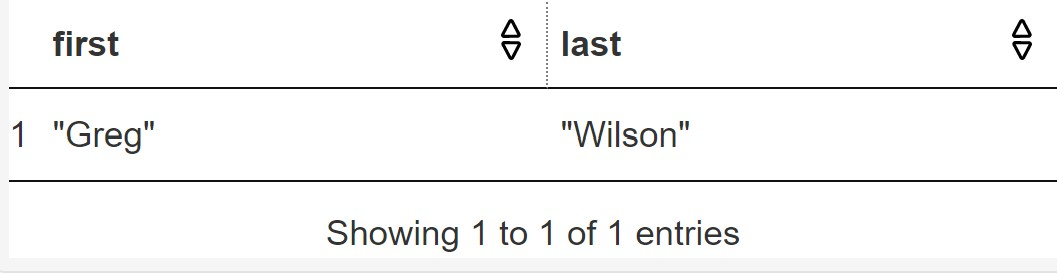
\includegraphics{images/12.jpg}
  \end{problem}

  \begin{problem}{4.4}
    \begin{verbatim}
PREFIX ex: <http://example.org/addressbook#>
PREFIX d: <http://example.org/data#>

INSERT { ?s ex:homeTel "(860) 578-7614" }
WHERE { 
  ?s ?p ?o.
  MINUS { ?s ex:homeTel ?x }
}
    \end{verbatim}

    \pagebreak
    Final Graph (also included in attachments):
    \begin{verbatim}
@prefix ex:    <http://example.org/addressbook#> .
@prefix d:     <http://example.org/data#> .

d:i55   a             ex:Student ;
        ex:email      "ElizabethMHolland@gmail.com" ;
        ex:firstName  "Elizabeth" ;
        ex:homeTel    "(802) 245-5788" ;
        ex:lastName   "Holland" .

d:i44   a             ex:Student ;
        ex:email      "GeorgeMWesterlund@gmail.com" ;
        ex:firstName  "George" ;
        ex:homeTel    "(414) 344-1585" ;
        ex:lastName   "Westerlund" .

d:i33   a             ex:Student ;
        ex:email      "greg@gmail.com" , "greg@yahoo.com" ;
        ex:firstName  "Greg" ;
        ex:homeTel    "(860) 578-7614" ;
        ex:lastName   "Wilson" .

d:i22   a             ex:Student ;
        ex:email      "emi@gmail.com" ;
        ex:firstName  "Emi" ;
        ex:homeTel    "(860) 846-2323" ;
        ex:lastName   "Smith" .

d:i11   a             ex:Student ;
        ex:email      "bob@hotmail.com" ;
        ex:firstName  "Bob" ;
        ex:homeTel    "(560) 333-5135" ;
        ex:lastName   "Jones" .

    \end{verbatim}
  \end{problem}
\end{document}